\subsection{Metric Outer Measures and Hausdorff Measure}

Metric outer measures are outer measures whose additivity recognizes positive separation. They abstract the positive-distance additivity of Euclidean cell-cover outer measure from Theorem \ref{thm:outer-measure-positive-distance-additivity}.

\begin{definition} \label{def:metric-caratheodory-outer-measure} \hlt{Metric/Caratheodory Outer Measure}\\
Let $(X,d)$ be a metric space and let $\omega:2^X\to[0,+\infty]$ be an outer measure.
\begin{enumerate}[label=(\roman*)]
\setlength{\itemsep}{0pt}
\item For nonempty $A,B\subseteq X$, $\operatorname{dist}(A,B)\defeq\inf\{d(a,b):a\in A,\ b\in B\}$.
\item $\omega$ is \hlt{metric outer measure} if $\operatorname{dist}(A,B)>0\Rightarrow\omega(A\cup B)=\omega(A)+\omega(B)$ $\forall$ nonempty $A,B\subseteq X$.
\end{enumerate}
\hlt{Key Insight}: Positive metric separation forces outer-measure additivity.
\end{definition}

\begin{definition} \label{def:real-function-separated-sets} \hlt{Separation by a Real-Valued Function}\\
Let $X$ be a set and let $\varphi:X\to\R$. Sets $A,B\subseteq X$ are \hlt{$\varphi$-separated} if, for some $r<s$, one of $A,B$ is contained in $\{\varphi\leq r\}$ and the other is contained in $\{\varphi\geq s\}$.
\end{definition}

\begin{proposition} \label{prop:function-separated-outer-measure-measurability} \hlt{Separation by One Real-Valued Function}\\
Let $X$ be a set, let $\omega:2^X\to[0,+\infty]$ be an outer measure, and let $\varphi:X\to\R$. If $\omega(A\cup B)=\omega(A)+\omega(B)$ for every $\varphi$-separated pair $A,B\subseteq X$, then $\varphi:(X,\mathcal{M}_\omega)\to(\R,\mathcal{B}(\R))$ is measurable.
\begin{proof} Fix $t\in\R$, put $E_t\defeq\{\varphi>t\}$, and fix $A\subseteq X$ with $\omega(A)<+\infty$. Set $B\defeq A\cap E_t$ and $C\defeq A\setminus E_t$.\\
For $n\geq1$, let $B_n\defeq A\cap\{\varphi>t+\frac{1}{n}\}$, $B_0\defeq\emptyset$, and $R_n\defeq B_n\setminus B_{n-1}$.\\
Same-parity strips are pairwise $\varphi$-separated, so $\sum\limits_{n\geq1}\omega(R_n)<+\infty$. Given $\varepsilon>0$, choose $n$ with $\sum\limits_{k>n}\omega(R_k)<\varepsilon$.\\
Since $B\subseteq B_n\cup\bigcup\limits_{k>n}R_k$ and $B_n,C$ are $\varphi$-separated, $\omega(B)+\omega(C)\leq\omega(B_n\cup C)+\varepsilon\leq\omega(A)+\varepsilon$.\\
Let $\varepsilon\downarrow0$, then $\omega(A)\geq\omega(A\cap E_t)+\omega(A\setminus E_t)$; Lemma \ref{lem:caratheodory-finite-measure-test} gives $E_t\in\mathcal{M}_\omega$ for every $t$, hence $\varphi$ is measurable.\\
\hlt{Structural Commentary}: Measurability reduces to a finite-mass split of each level set.\\
\hlt{Key Insight}: Summable level strips leave an arbitrarily small boundary layer.
\end{proof}
\end{proposition}

\begin{theorem} \label{thm:metric-outer-measure-borel-measurable} \hlt{Metric Outer Measures Measure Borel Sets}\\
Let $(X,d)$ be a metric space and let $\omega:2^X\to[0,+\infty]$ be a metric outer measure. Then:
\begin{enumerate}[label=(\roman*)]
\setlength{\itemsep}{0pt}
\item Every closed $F\subseteq X$ belongs to $\mathcal{M}_\omega$.
\item $\mathcal{B}(X)\subseteq\mathcal{M}_\omega$.
\end{enumerate}
\begin{proof}
\begin{enumerate}[label=(\roman*)]
\setlength{\itemsep}{0pt}
\item The case $F=\emptyset$ is immediate. For nonempty closed $F$, set $\varphi(x)\defeq\operatorname{dist}(\{x\},F)$. Proposition \ref{prop:distance-to-set-is-continuous} gives $\varphi$ $1$-Lipschitz and $F=\varphi^{-1}(\{0\})$, so $\varphi$-separated pairs have positive distance. Metric additivity verifies Proposition \ref{prop:function-separated-outer-measure-measurability}; hence $\varphi$ is $\mathcal{M}_\omega$-measurable and $F\in\mathcal{M}_\omega$.
\item By (i), all closed sets lie in the $\sigma$-algebra $\mathcal{M}_\omega$; since they generate $\mathcal{B}(X)$, $\mathcal{B}(X)\subseteq\mathcal{M}_\omega$.
\end{enumerate}
\hlt{Structural Commentary}: Distance functions turn closed sets into real-valued separation tests.\\
\hlt{Key Insight}: Closed measurability plus generation gives Borel measurability.
\end{proof}
\end{theorem}

\begin{definition} \label{def:hausdorff-outer-measure} \hlt{Hausdorff Outer Measure}\\
Let $(X,d)$ be a metric space, $\alpha>0$, $\varepsilon>0$.
\begin{enumerate}[label=(\roman*)]
\setlength{\itemsep}{0pt}
\item $\mathcal{H}_{\alpha,\varepsilon}^\ast(\emptyset)\defeq0$; $\mathcal{H}_{\alpha,\varepsilon}^\ast(E)\defeq\inf\{\sum\limits_{k=1}^{\infty}(\diam A_k)^\alpha:E\subseteq\bigcup\limits_{k=1}^{\infty}A_k,\ \emptyset\neq A_k\subseteq X,\ \diam A_k<\varepsilon\}$, nonempty $E\subseteq X$
\item If $0<\varepsilon_1<\varepsilon_2$, then $\mathcal{H}_{\alpha,\varepsilon_1}^\ast(E)\geq\mathcal{H}_{\alpha,\varepsilon_2}^\ast(E)$.
\item $\mathcal{H}_\alpha^\ast(E)\defeq\sup_{\varepsilon>0}\mathcal{H}_{\alpha,\varepsilon}^\ast(E)=\lim_{\varepsilon\downarrow0}\mathcal{H}_{\alpha,\varepsilon}^\ast(E)$.
\end{enumerate}
\hlt{Key Insight}: $\mathcal{H}_\alpha^\ast$ is the limiting cost of countable small-diameter covers.
\end{definition}

\begin{figure}[H]
  \centering
  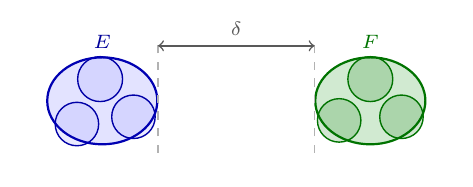
\begin{tikzpicture}[
  scale=0.92,
  every node/.style={font=\scriptsize},
  setEfill/.style={fill=blue!55, fill opacity=0.20, draw=none},
  setFfill/.style={fill=green!55!black, fill opacity=0.18, draw=none},
  setEline/.style={draw=blue!70!black, line width=0.8pt},
  setFline/.style={draw=green!45!black, line width=0.8pt},
  coverE/.style={fill=blue!35, fill opacity=0.23, draw=blue!65!black, line width=0.5pt},
  coverF/.style={fill=green!45!black, fill opacity=0.18, draw=green!45!black, line width=0.5pt},
  guide/.style={draw=gray!60, dashed, line width=0.45pt},
  measure/.style={<->, gray!70!black, line width=0.55pt}
]
  \path[use as bounding box] (-2.88,-0.76) rectangle (2.88,1.05);

  \path[setEfill] (-1.85,0.04) ellipse [x radius=0.76, y radius=0.60];
  \path[setFfill] (1.85,0.04) ellipse [x radius=0.76, y radius=0.60];

  \draw[coverE] (-2.20,-0.28) circle [radius=0.30];
  \draw[coverE] (-1.88,0.34) circle [radius=0.31];
  \draw[coverE] (-1.42,-0.18) circle [radius=0.30];

  \draw[coverF] (1.42,-0.23) circle [radius=0.30];
  \draw[coverF] (1.85,0.34) circle [radius=0.31];
  \draw[coverF] (2.28,-0.18) circle [radius=0.30];

  \draw[setEline] (-1.85,0.04) ellipse [x radius=0.76, y radius=0.60];
  \draw[setFline] (1.85,0.04) ellipse [x radius=0.76, y radius=0.60];

  \draw[guide] (-1.08,-0.68) -- (-1.08,0.90);
  \draw[guide] (1.08,-0.68) -- (1.08,0.90);
  \draw[measure] (-1.08,0.80) -- (1.08,0.80)
    node[midway, above] {$\delta$};

  \node[blue!60!black] at (-1.85,0.86) {$E$};
  \node[green!45!black] at (1.85,0.86) {$F$};
\end{tikzpicture}

  \caption{$\operatorname{dist}(E,F)=\delta$ and $\diam A_k<\delta$: each $A_k$ meets at most one of $E,F$.}
  \label{fig:hausdorff-separated-cover-split}
\end{figure}

\begin{theorem} \label{thm:hausdorff-measure-borel-construction} \hlt{Hausdorff Measure on Borel Sets}\\
Let $(X,d)$ be a metric space and let $\alpha>0$. Then:
\begin{enumerate}[label=(\roman*)]
\setlength{\itemsep}{0pt}
\item $\mathcal{H}_\alpha^\ast:2^X\to[0,+\infty]$ is a metric outer measure.
\item $\mathcal{H}_\alpha\defeq\mathcal{H}_\alpha^\ast|_{\mathcal{B}(X)}$ is a measure on $\mathcal{B}(X)$, called the \hlt{$\alpha$-dimensional Hausdorff measure} on $X$.
\end{enumerate}
\begin{proof}
\begin{enumerate}[label=(\roman*)]
\setlength{\itemsep}{0pt}
\item For each $\varepsilon>0$, $\mathcal{H}_{\alpha,\varepsilon}^\ast(\emptyset)=0$, monotonicity is immediate from admissible covers, and countable subadditivity follows by joining admissible $\varepsilon$-covers; hence $\mathcal{H}_\alpha^\ast(\bigcup\limits_i E_i)=\sup\limits_{\varepsilon>0}\mathcal{H}_{\alpha,\varepsilon}^\ast(\bigcup\limits_i E_i)\leq\sum\limits_i\mathcal{H}_\alpha^\ast(E_i)$.\\
Thus $\mathcal{H}_\alpha^\ast$ is an outer measure. If $\operatorname{dist}(E,F)=\delta>0$ and $0<\varepsilon<\delta$, every admissible $\varepsilon$-cover of $E\cup F$ splits into disjoint subcovers of $E$ and $F$, so $\mathcal{H}_{\alpha,\varepsilon}^\ast(E\cup F)\geq\mathcal{H}_{\alpha,\varepsilon}^\ast(E)+\mathcal{H}_{\alpha,\varepsilon}^\ast(F)$.\\
Letting $\varepsilon\downarrow0$ and using subadditivity gives metric additivity.
\item By (i), $\mathcal{H}_\alpha^\ast$ is a metric outer measure; Theorem \ref{thm:metric-outer-measure-borel-measurable} gives $\mathcal{B}(X)\subseteq\mathcal{M}_{\mathcal{H}_\alpha^\ast}$.\\
Since $\mathcal{H}_\alpha^\ast|_{\mathcal{M}_{\mathcal{H}_\alpha^\ast}}$ is a measure, its restriction $\mathcal{H}_\alpha^\ast|_{\mathcal{B}(X)}=\mathcal{H}_\alpha$ is a measure on $\mathcal{B}(X)$.
\end{enumerate}
\hlt{Structural Commentary}: Cover infima give the outer measure; separated cover splitting gives metric additivity.\\
\hlt{Key Insight}: Small-diameter covers cannot straddle positive gaps.
\end{proof}
\end{theorem}

\begin{example} \label{ex:hausdorff-measure-finite-sets} \hlt{Finite Sets Have Zero Positive-Dimensional Hausdorff Measure}\\
If $E=\{x_1,\ldots,x_N\}\subseteq X$ and $\alpha>0$, then $\mathcal{H}_\alpha^\ast(E)=0$: for every $\varepsilon>0$, the singleton cover $E\subseteq\bigcup\limits_{j=1}^{N}\{x_j\}$ is admissible and has total $\alpha$-content $\sum\limits_{j=1}^{N}(\diam\{x_j\})^\alpha=0$.\\
\hlt{Key Insight}: Finite sets are covered by zero-diameter singletons.
\end{example}

\begin{proposition} \label{prop:hausdorff-measure-critical-exponent} \hlt{Hausdorff Measures Decrease Through Dimension}\\
Let $(X,d)$ be a metric space, let $E\subseteq X$, and let $0<\alpha<\beta$. If $\mathcal{H}_\alpha^\ast(E)<+\infty$, then $\mathcal{H}_\beta^\ast(E)=0$.
\begin{proof} Fix $\varepsilon>0$. Choose admissible $\varepsilon$-cover $(A_k)$ of $E$ with $\sum\limits_k(\diam A_k)^\alpha\leq\mathcal{H}_{\alpha,\varepsilon}^\ast(E)+1\leq\mathcal{H}_\alpha^\ast(E)+1$.\\
Since $\diam A_k<\varepsilon$, $\sum\limits_k(\diam A_k)^\beta=\sum\limits_k(\diam A_k)^{\beta-\alpha}(\diam A_k)^\alpha\leq\varepsilon^{\beta-\alpha}(\mathcal{H}_\alpha^\ast(E)+1)$.\\
Hence $\mathcal{H}_{\beta,\varepsilon}^\ast(E)\leq\varepsilon^{\beta-\alpha}(\mathcal{H}_\alpha^\ast(E)+1)$. Letting $\varepsilon\downarrow0$ gives $\mathcal{H}_\beta^\ast(E)=0$.\\
\hlt{Structural Commentary}: Compare one small cover at dimensions $\alpha$ and $\beta$.\\
\hlt{Key Insight}: The factor $\varepsilon^{\beta-\alpha}$ kills finite $\alpha$-content.
\end{proof}
\end{proposition}

\begin{definition} \label{def:hausdorff-dimension} \hlt{Hausdorff Dimension}\\
For $E\subseteq X$, the \hlt{Hausdorff dimension} is $\dim_H(E)\defeq\inf\{\beta>0:\mathcal{H}_\beta^\ast(E)=0\}$, with $\inf\emptyset\defeq+\infty$.
\end{definition}

\begin{remark} \label{rem:hausdorff-dimension-threshold} \hlt{Dimension as a Critical Exponent}\\
For $E\subseteq X$, set $Z_E\defeq\{\beta>0:\mathcal{H}_\beta^\ast(E)=0\}$. Proposition \ref{prop:hausdorff-measure-critical-exponent} gives $Z_E=(\dim_H(E),+\infty)$ or $[\dim_H(E),+\infty)$ inside $(0,+\infty)$, so $\dim_H(E)$ is the zero-measure threshold for the Hausdorff scale.
\end{remark}

\begin{remark} \label{rem:hausdorff-one-dimensional-calibration} \hlt{One-Dimensional Calibration}\\
On $\R$, interval covers give $\mathcal{H}_1^\ast((a,b])\leq b-a$, and every diameter cover of $(a,b]$ enlarges to interval covers with arbitrarily small extra total length, giving $\mathcal{H}_1^\ast((a,b])\geq b-a$. Hence $\mathcal{H}_1^\ast((a,b])=b-a$, and uniqueness of the Borel extension from half-open intervals gives $\mathcal{H}_1=m$ on $\mathcal{B}(\R)$.
\end{remark}
